% Pizza casera
\newpage
\begin{recipe}[source={La Mami},
portion={2-6 personas},
preparationtime={\unit[1]{Hora}}
]{Pizza Casera}
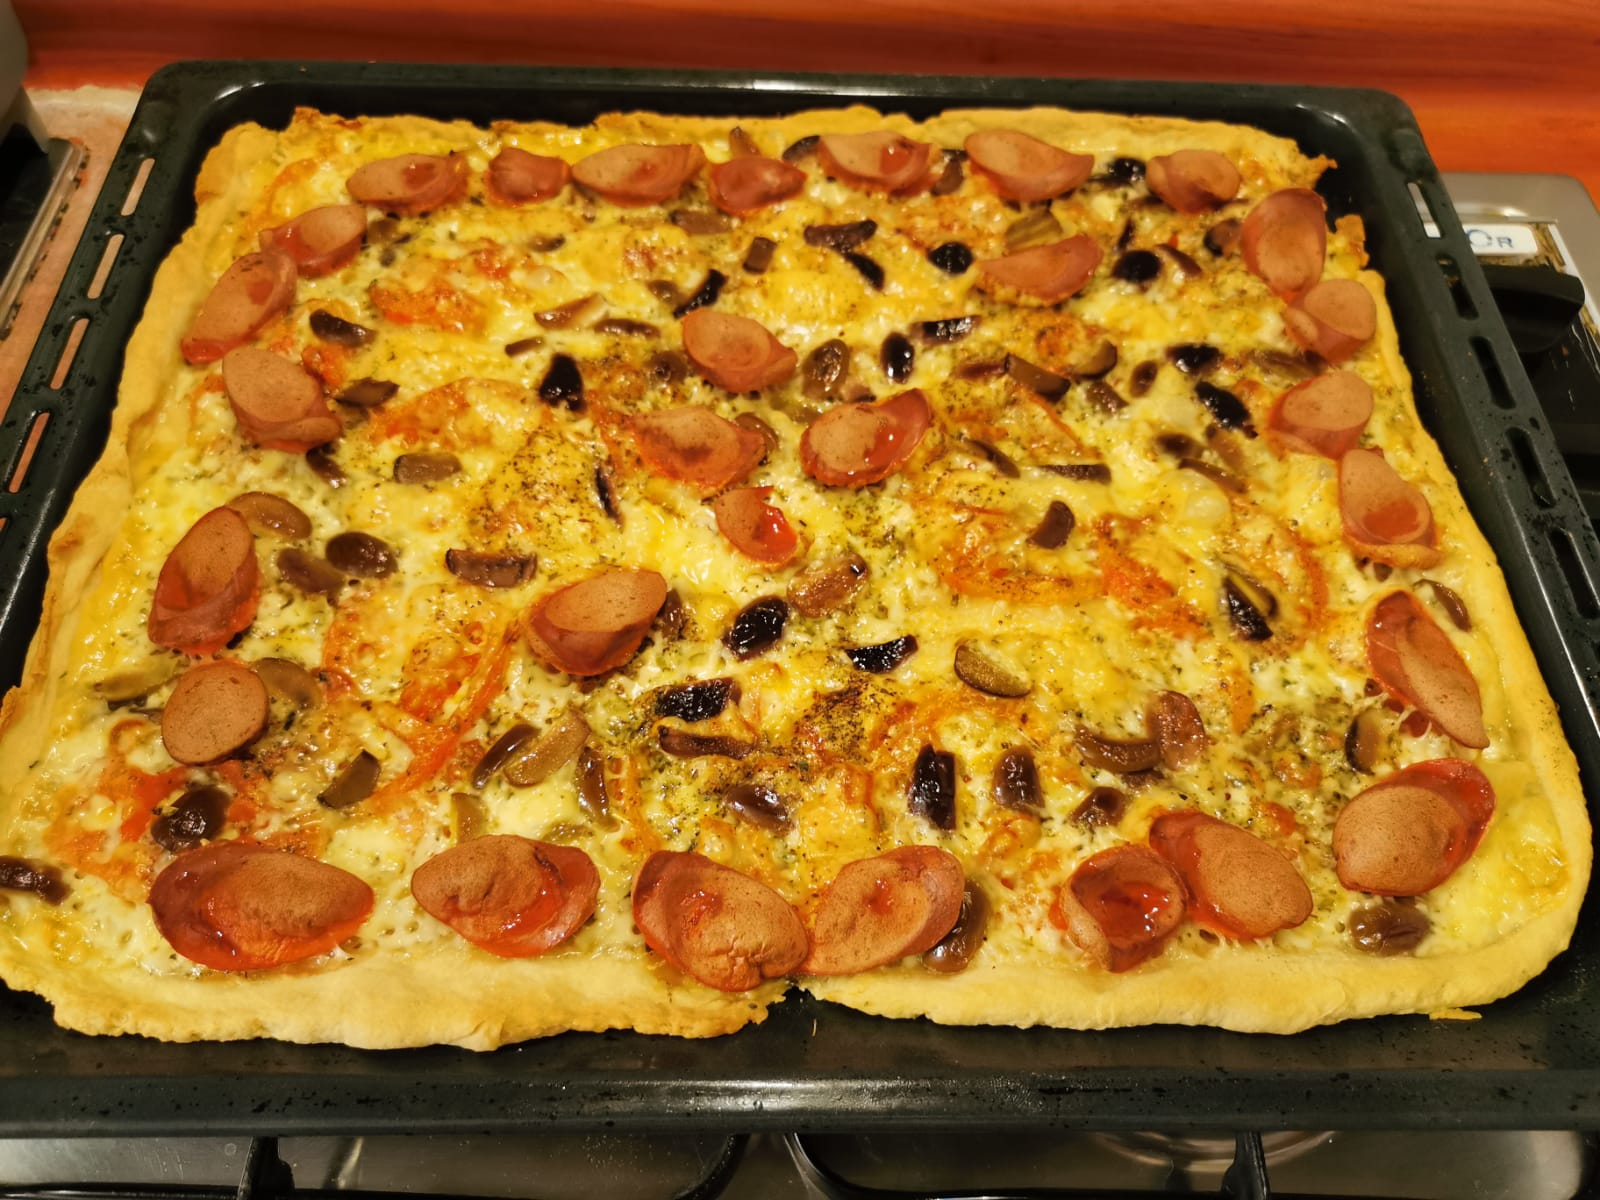
\includegraphics[width=0.25\textwidth]{pizza}
\introduction{
A quién no le gusta la pizza. Siempre son bienvenidas en cualquier momento y hora.
}
\ingredients{
	& \textbf{Para la masa:} \\
    4 & tazas de harina \\
    1 & cucharada de polvos de hornear \\
    1 & cucharadita de sal \\
    2 & cucharadas de aceite de oliva \\
    1 & taza de agua tibia o leche \\
    & \textbf{Para el acompañamiento:} \\
    2 & tomates cortados en rodajas finas \\
    \unit[500]{gr} & de queso laminado \\
    \unit[250]{gr} & de aceitunas \\
    \unit[100]{gr} & de salame \\
    & Orégano a gusto
}
\preparation{
    \begin{enumerate}
        \item Preparar la masa en un bol integrando la harina, la sal, el aceite, los polvos de hornear y poco a poco el agua.
        \item Pre calentar el horno por 5 minutos a 180 grados con calor arriba y abajo.
        \item Estirar la masa en la bandeja previamente aceitada.
        \item Colocar el tomate, el queso, el orégano, el salame y las aceitunas.
        \item Meter la bandeja al horno y cocinar por aproximadamente unos 30-40 minutos o hasta que los bordes de la masa estén dorados.
        \item Retirar y servir.
    \end{enumerate}
}
\hint{
	Puedes echar un poco de merquén si te gusta que tenga un condimento picante.
}

\end{recipe}